%   *******************************************************************
%   * THIS IS THE MAIN FILE--RUNNING LATEX ON "AllegThesis.tex" WILL  *
%   * GENERATE THE ENTIRE THESIS (ASSUMING YOU HAVE NOT RENAMED IT).  *
%   * IF YOU ARE USING BIBTEX, RUNNING BIBTEX ON "AllegThesis" SHOULD *
%   * GENERATE YOUR BIBLIOGRAPHY. SPECIFIC DETAILS DEPEND ON WHAT     *
%   * ENVIRONMENT AND TOOLS YOU ARE USING (E.G., TEXMAKER OR COMMAND  *
%   * LINE TOOLS LIKE PDFLATEX OR ...).                               *
%   *******************************************************************
%
% AllegThesis.tex
% by Braden Licastro
% 13 Feb 2003
%
% Revised by R. Roos
% Nov 2013
%
% This document provides a sample Senior Thesis template for use
% by students in Allegheny's CS and Applied Computing programs.
%
%   *******************************************************************
%   * LOOK FOR BLOCK COMMENTS SUCH AS THIS ONE FOR AN EXPLANATION OF  *
%   * THIS DOCUMENT AND HOW TO MODIFY IT FOR YOUR OWN THESIS!         *
%   *                                                                 *
%   * ANY LINE BEGINNING WITH A "%" IS A LATEX COMMENT AND IS IGNORED *
%   * BY THE LATEX PROCESSOR. YOU ARE ENCOURAGED TO COMMENT YOUR OWN  *
%   * LATEX CODE TO HELP YOU REMEMBER WHY YOU DID THINGS A CERTAIN WAY*
%   *******************************************************************
%

%   ********************************************************************
%   * THE FIRST SECTION OF THE MAIN LATEX FILE IS THE "PREAMBLE." IT   *
%   * INSTRUCTS LATEX TO IMPORT SPECIAL PACKAGES FOR THINGS LIKE       *
%   * INCLUDING FIGURES, DOUBLE-SPACING, COLORED TEXT, ETC.            *
%   * DEPENDING ON YOUR NEEDS, YOU MAY FIND IT NECESSARY TO USE PACK-  *
%   * AGES THAT ARE NOT INCLUDED IN THIS TEMPLATE. SIMPLY IMITATE THE  *
%   * "\usepackage{...}" COMMANDS SHOWN BELOW.                         *
%   ********************************************************************

%   ********************************************************************
%   * BEGINNING OF PREAMBLE:                                           *
%   ********************************************************************

\NeedsTeXFormat{LaTeX2e}
\documentclass[12pt]{report}

%   ********************************************************************
%   * ALL BUT ONE OF THE FOLLOWING 5 LINES SHOULD BE COMMENTED OUT.    *
%   * (NOT ALL OF THESE OPTIONS HAVE BEEN TESTED IN THIS REVISION!)    *
%   ********************************************************************

%\usepackage[debug,draft,double]{gatorthesis} % for student proof doublespace
\usepackage[bottom,double]{gatorthesis} % for final department copy
%\usepackage[debug,draft,single]{gatorthesis} % for student workcopy
%\usepackage[single]{gatorthesis} % for student
%\usepackage[debug,draft,nolists,nofront,single]{gatorthesis} % more options


\usepackage{comment}     % provides a way to "comment out" sections in blocks
\usepackage{doublespace} % final document should be double-spaced!
\usepackage{amsmath}     % special symbols
\usepackage{amssymb}     % more special symbols
\usepackage{epsfig}      % needed for including figures
% \usepackage{fancybox}  % --- DISABLED BY RSR, SEP 2013 ---
\usepackage{listings}
\usepackage{xcolor}
\usepackage[figure]{algorithm2e}
\usepackage{graphicx}
\usepackage{epstopdf}
\epstopdfsetup{update} % only regenerate pdf files when eps file is newer
\usepackage[hyphens]{url}

\definecolor{dkgreen}{rgb}{0,.6,0}
\definecolor{dkblue}{rgb}{0,0,.6}
\definecolor{dkyellow}{cmyk}{0,0,.8,.3}

%   ********************************************************************
%   * OPTIONAL: IF YOU WANT VERY FINE CONTROL OVER HOW LATEX HYPHENATES*
%   * CERTAIN WORDS, YOU CAN PUT WORDS IN A "\hyphenation" COMMAND AS  *
%   * SHOWN IN THE FOLLOWING EXAMPLE. OTHERWISE, YOU MAY JUST IGNORE   *
%   * THE NEXT COMMAND.                                                *
%   ********************************************************************

% EXAMPLE: Don't hyphenate the words "itself" or "linear". Hyphenate 
%          "representations" only at the places indicated by the "-":

\hyphenation{itself repre-sen-tations linear}

%   ********************************************************************
%   * THE FOLLOWING COMMAND HAS BEEN DISABLED--IGNORE.                 *
%   ********************************************************************
% The following provides a box to surround the thesis statement
%\newenvironment{Thesis}%
%{\begin{Sbox}\begin{minipage}{.95\linewidth}}%
%{\end{minipage}\end{Sbox}\begin{center}\fbox{\TheSbox}\end{center}}

%   ********************************************************************
%   ********************************************************************
%   ***  END OF PREAMBLE.                                            ***
%   ********************************************************************
%   ********************************************************************



%   ********************************************************************
%   * DOCUMENT CONTENT STARTS AT THE "\begin{document}" COMMAND:       *
%   ********************************************************************

\begin{document}

%   ***********************************
%   *         MY INFORMATION.         *
%   ***********************************

\thesistitle{Approximate Algorithmic Image Matching to Reduce Online Storage Overhead of User Submitted Images}

\thesisauthor{Braden D. Licastro} \thesisadvisor{Dr. Robert Roos}

\thesisnumber{CS14-11} % REPORT NUMBER PROVIDED BY PAULINE LANZINE!

\thesisreadera{Dr. Gregory Kapfhammer}


%   ********************************************************************
%   * IN RARE CASES YOU MAY HAVE MORE THAN TWO READERS, IN WHICH CASE  *
%   * YOU SHOULD UN-COMMENT THE FOLLOWING AND ADD NAMES:               *
%   ********************************************************************
% \thesisreaderb{Dr. Your Thirdreader} 
% \thesisreaderc{Dr. Your Fourthreader}
% \thesisreaderd{Dr. Your Fifthreader}

%   ********************************************************************
%   * YOU MAY IGNORE THE FOLLOWING COMMAND:                            *
%   ********************************************************************
\date{\FileRevised \\ $\mbox{}$Revision: 1.8 $\mbox{}$}

\thesismaketitle         % Creates the title page
\thesismakecopyright     % Creates the copyright page

%   ********************************************************************
%   * YOU MAY SPLIT YOUR THESIS INTO SEVERAL FILES AND "\include" THEM *
%   * AS SHOWN BELOW. FOR INSTANCE, FILE "abstract.tex" CONTAINS THE   *
%   * ABSTRACT, FILE "ack.tex" CONTAINS THE ACKNOWLEDGMENTS, ETC. YOU  *
%   * MAY, OF COURSE, PUT EVERYTHING INTO ONE HUGE FILE, BUT THERE ARE *
%   * ADVANTAGES TO SPLITTING THINGS UP--FOR EXAMPLE, YOU CAN COMMENT  *
%   * OUT "\include" LINES OF SOME PARTS IN ORDER TO PRINT DRAFTS      *
%   * CONTAINING SELECTED SECTIONS OF YOUR THESIS, SAVING PAPER AND    *
%   * PRINTING COSTS.                                                  *
%   *                                                                  *
%   * YOU ARE NOT REQUIRED TO HAVE A "dedication"--IF YOU DON'T, JUST  *
%   * DELETE THAT LINE OR COMMENT IT OUT WITH A LEADING "%"            *
%   ********************************************************************

\begin{abstract}
Reducing the number of duplicate images uploaded to public servers is an ever more relevant problem as the number of images shared increases dramatically every day. Methods of data reduction such as file expiration dates only lessen this load by a small amount while common methods of image matching are in many cases resource exhaustive, time consuming, or highly inaccurate. This research utilizes technologies capable of identifying near-duplicate images through file hashing, pixel difference, and histogram comparisons. In order to evaluate the feasibility of implementing such a system, a basic photo sharing website has been developed and run on a fixed collection of images. This system was then empirically evaluated with a focus on accuracy and performance with results suggesting acceptable performance and detection rates.
\end{abstract}
  % REQUIRED!

%
% $Id: dedication
%
%   *******************************************************************
%   * SEE THE MAIN FILE "AllegThesis.tex" FOR MORE INFORMATION.       *
%   *******************************************************************
\begin{dedication}
\vspace*{.68in}
    \begin{Huge}
        \textbf{Dedication\\}
        \vspace{.355in}
    \end{Huge}

To Professor Cupper. He was more than just an advisor and professor; he was a member of the Alden family and a father away from home.
\end{dedication} % OPTIONAL

%
% $Id: ack
%
%   *******************************************************************
%   * SEE THE MAIN FILE "AllegThesis.tex" FOR MORE INFORMATION.       *
%   *******************************************************************
\clearpage
\thispagestyle{plain}
\chapter*{Acknowledgements}
I would like to thank my thesis advisor, Professor Roos for the time, expertise, and guidance he provided me as I worked through this project. I would also like to thank my family and girlfriend for their support and encouragement that kept me going until the end.       % OPTIONAL, BUT ALMOST EVERYONE INCLUDES IT

%   ********************************************************************
%   * FRONT MATTER--TABLE OF CONTENTS, ETC. YOU PROBABLY DON'T NEED TO *
%   * CHANGE ANY OF THIS UNLESS YOU HAVE NO TABLES OR FIGURES, OR YOU  *
%   * WANT TO CHANGE NUMBERING DEPTH FOR SUBSECTIONS, OR ...           *
%   ********************************************************************

\setcounter{tocdepth}{2}    % # of section levels shown in table of contents
\setcounter{secnumdepth}{3} % # of numbered subsection levels in the text

\tableofcontents
%\listoftables       % OMIT THIS IF YOU DON'T HAVE ANY TABLES
\listoffigures      % OMIT THIS IF YOU DON'T HAVE ANY FIGURES

%   ********************************************************************
%   * A GLOSSARY IS ALMOST NEVER NEEDED UNLESS YOU HAVE AN UNUSUALLY   *
%   * LARGE NUMBER OF SPECIAL TERMS OR NOTATIONS AND IT WOULD DETRACT  *
%   * TOO MUCH FROM THE FLOW OF THE PAPER TO DEFINE THEM IN-LINE.      *
%   ********************************************************************
%\include{glossary}  % OMIT THIS IF YOU DON'T HAVE A GLOSSARY (FEW PEOPLE DO)


%   ********************************************************************
%   * THE FOLLOWING "lstset" COMMAND IS ADAPTED FROM ONE FOUND AT:     *
%   * http://tex.stackexchange.com/questions/115467/                   *
%   * listings-highlight-java-annotations                              *
%   *                                                                  *
%   * SEE CHAPTER 3 AND APPENDIX A                                     *
%   ********************************************************************

%\lstset{
%  basicstyle=\footnotesize\tt, % the size of the fonts that are used for the code
%  breakatwhitespace=false,     % automatic breaks only happen at whitespace?
%  breaklines=true,             % sets automatic line breaking
%  captionpos=b,                % sets the caption-position to bottom
%  frame=single,                % adds a frame around the code
%  language=Java,               % the language of the code
%  keywordstyle=\bf,
%  showspaces=false,
%  showstringspaces=false,      % underline spaces within strings only?
%  showtabs=false,
%  tabsize=2                    % sets default tabsize to 2 spaces
%}


%   ********************************************************************
%   * NOW INCLUDE THE CHAPTER FILES; COMMENT OUT ANY YOU DON'T WANT TO *
%   * PROCESS IN A PARTICULAR LATEX RUN.                               *
%   *                                                                  *
%   * INCLUDED FILES ARE ASSUMED TO END IN ".tex", E.G.,               *
%   * "ch01_overview.tex", "ch02_relatedwork.tex", ETC.                *
%   ********************************************************************

% ch:intro
%
% $Id: ch01_overview
%
%   *******************************************************************
%   * SEE THE MAIN FILE "AllegThesis.tex" FOR MORE INFORMATION.       *
%   *******************************************************************

\chapter{Introduction}\label{ch:intro} % we can refer to chapter by the label

%   ************************************************************************
%   * In LaTeX, new paragraphs are begun by simply leaving a blank line in *
%   * the LaTeX file.                                                      *
%   *                                                                      *
%   * The \\ characters should NEVER be used to end a paragraph.           *
%   * They are used only for inserting line breaks in certain situations.  *
%   *                                                                      *
%   * "Widows" (ending paragraph lines at the top of a new page) and       *
%   * "orphans" (opening paragraph lines at the bottom of a page) should   *
%   * be eliminated; this sometimes requires re-writing some of the        *
%   * text to change the line lengths.                                     *
%   ************************************************************************

Sharing media with the public is becoming a more integral part of social interaction every day. Static images are just one of these many forms of media, and the number of daily uploads to image hosting websites is absolutely staggering. According to a recent survey by All Things Digital, as of May 2013, more than 500 million images are uploaded to image sharing websites each day, and this number is expected to double by the end of 2014 \cite{meek:500}. With figures this large, it immediately becomes apparent that multiple issues come with this trend of increased image sharing, namely, how much space does this number of images require, and is there a technology available to reduce this requirement? The simple answer is yes, there are tried and tested technologies that will reduce storage costs, but before looking into these technologies, it is important to understand what an image hosting website is and how they function.

\section{Image Hosting Services} \label{sec:imagehostingservices}
Image hosting services, or image sharing websites, are sites that allow users to upload images to the internet and share them publicly with the link they are provided. These image sharing websites mostly operate in the same fashion, but recently a new breed has emerged. As seen in Figure \ref{imageshareprocess}, both submission processes are similar, but both have inherent advantages and disadvantages.

\begin{figure}[htbp]
\centering
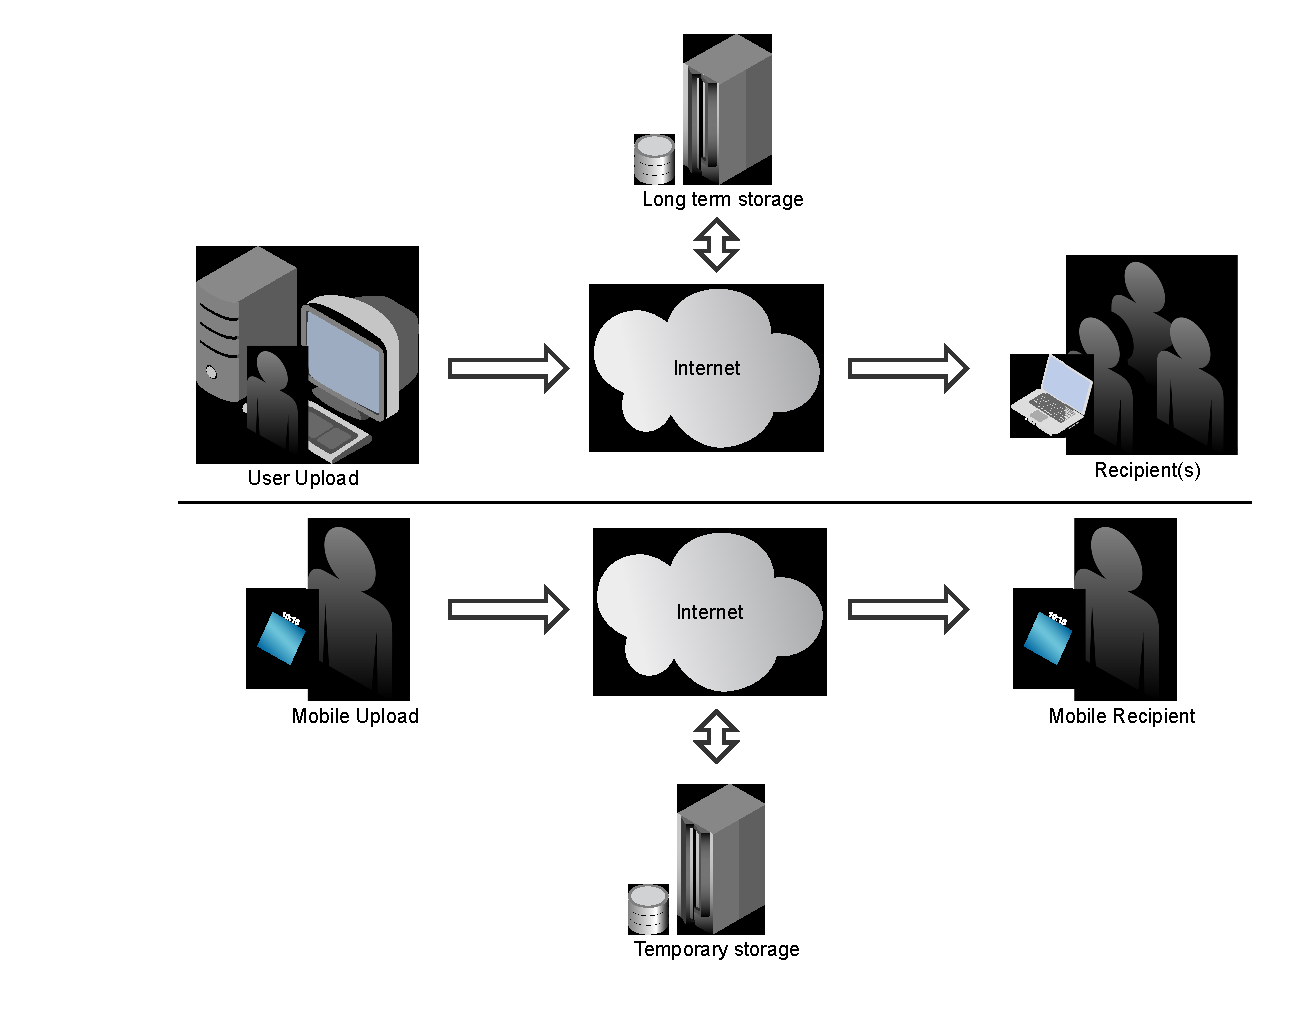
\includegraphics[width=4.5in]{imageshareprocess}
\caption{Various Image Hosting Service Structures}
\label{imageshareprocess}
\end{figure}

Looking at the first submission process variant at the top of Figure \ref{imageshareprocess}, a user would like to share an image with the public. The user can upload this image through the internet from any internet connected device, and the image will be stored on a publicly accessible server. From here, any number of people can access this shared image through an internet connected device indefinitely. Nearly all image hosting services operate on this model, some of the more popular services include but are not limited to Flickr, Imgur, Photobucket, Shutterfly, and Instagram.

The second image submission variant shown at the bottom half of Figure \ref{imageshareprocess} is currently only used by one host called Snapchat. With this system, multiple differences are immediately apparent. First, this service model will only accept images from mobile users. It can also be seen in the diagram that when a user uploads an image through the internet, it is no longer accessible long term from a server, but it is in fact only temporarily available for a specified recipient to receive. This service actually allows the uploader to set an expiration time anywhere from 1 second to 10 seconds \cite{snap:support}. After the recipient opens the image and this time period has expired, the image is deleted permanently from the server and no longer accessible to either party.

Both systems have their own inherent benefits, but they also have drawbacks. Though they reach from the infrastructure needed to support the service all the way out to the end user, this research only focuses on the infrastructure function. In order to realize the application of the proposed research, it is important to understand why such a focused application is required. For the first image hosting variant in Figure \ref{imageshareprocess}, the long term storage of image files raises concern. By storing files for an extended period of time, it is a guarantee that duplicate data will eventually make its way to the storage servers. Determining duplicates and preventing their addition can save not only a considerable amount of space as the amount of redundant data increases, but it can also save a large amount of money when discussing the cost per gigabyte of data storage. This research will not target the application of the temporary system seen at the bottom of the figure as the amount of stored data is minimal due to the rapid turnover of data being housed.

\section{Data Management Technologies} \label{sec:datadeduptech}
The image hosting services outlined in section \ref{sec:imagehostingservices} utilize numerous technologies to help lessen the load of the files they must store. Though official word and articles discussing the technologies these companies implement are nonexistent, after examining the services several different technologies became immediately apparent. The most prominent method of space reduction is the reduction in size of uploaded images. By reducing the quality of the image by a small percent, these websites are able to significantly reduce the amount of space needed to store the uploaded images. The next most common method of space reduction used is the expiration of uploads. After locating the earliest available images across the websites it was determined that the file expiration can possibly work in one of two ways. The implementation either functions as a countdown from the date of upload or in the other case the countdown begins after the last date the file was accessed. Each time the file is accessed, the timer will reset. Finally, some of these sites also limit the size of the uploaded files and the number of uploads per user. In order to remove these restrictions, many sites also offer paid services which assist with the cost of upkeep. 

\section{Motivation} \label{sec:motivation}
Summarizing the information presented thus far, image hosting websites clearly require complex infrastructures, not only to allow the sharing of files but to manage the large numbers of submissions. Although the numerous technologies used to lessen the space requirements of the submissions work well, it should be possible to further improve on the system by reducing the number of duplicate submissions. According to a recent survey by All Things Digital, more than 500 million images are uploaded to long-term image sharing websites, and this number is expected to double by the end of 2014 \cite{meek:500}. In addition, a study published by NTP Software found that nearly 20\% of stored data is duplicate \cite{ntps:staledata}. These numbers are staggering, especially when there is a possibility of reducing an additional 100 million images.

To bring the possible savings into light a rough calculation based on the 2013 average of \$.05 per gigabyte and an assumed image size of 1MB will show that by removing the duplicates a significant amount of money could be saved. More specifically, approximately \$18 million can be saved annually at the current sharing levels. By allowing unregulated user submitted data, it quickly becomes apparent that data redundancy reduction can save a significant amount of storage space and money.

\section{Goals of the Project}\label{sec:goals}
The purpose of this project is to develop and test a system capable of identifying and reducing the number of duplicate image submissions on an image sharing website. In order to fulfill this goal, an image sharing website will be developed that is capable of accepting images as uploads and providing a link to the user for public access of the image. To develop a functional website it must be able to perform several functions. This website should accept an image file through an online submission form. At this point, it will process the image and match it against the collection of images currently stored on the server. This process will be completed using a series of algorithms and checks outlined in in section \ref{ch:method}. The website will also be developed using PHP, the PHP GD image library, and HTML5 to ensure minimal chance of conflicts between scripts and languages. Using this website, the proposed duplicate image detection tool will be implemented using both original and existing code from other resources and tested thoroughly to assess the effectiveness of using this method of duplicate reduction.

\section{Thesis Outline}\label{sec:outline}
The remainder of this thesis will discuss the work in further detail in addition to existing information relating to the topic. The first topic being discussed is Chapter \ref{ch:relatedwork}, which covers related works and existing research that has been completed on the topic of image matching and comparison. Chapter \ref{ch:method} will cover the project details pertaining to the website and supporting infrastructure it will operate on. This will include a brief discussion of the hardware and configuration of the web server in addition to the website design and implementation of the duplicate image detection tool that will be integrated and tested. Chapter \ref{ch:reseval} will then discuss the collected results and the accompanying evaluation of the collected data. This evaluation will include the performance costs of implementing this system over a passive one, which only acts to prevent a specific file from ever being submitted to the server. The evaluation will also include the results of the image de-duplication and a determination of whether such a system is a feasible method of reducing storage requirements. An additional section outlining threats to validity will also be included in this chapter. Finally, Chapter \ref{ch:conclusion} will summarize the research and conclusions completed throughout this Senior Comprehensive Project and include possible areas of future work. % Introduction -- of course, you can name it anything!

% ch:relatedwork
%
% $Id: ch02_relatedwork
%
%   *******************************************************************
%   * SEE THE MAIN FILE "AllegThesis.tex" FOR MORE INFORMATION.       *
%   *******************************************************************
\chapter{Related Work}\label{ch:relatedwork}

As expressed in the previous chapter, storage space on Internet accessible servers is at a premium when users have the ability to freely add content. In order to reduce the cost of operating image sharing websites it is necessary to develop and utilize technologies to reduce the space requirements. It is unsurprising that a large amount of research exists which targets the problem of locating similar images. Often, these comparison techniques were developed to be run on a local computer and not over the Internet, although the methods could be adapted to operate on a web based platform in many cases. By utilizing a combination of the research found in this chapter, it is possible to build a functional system capable of eliminating a large percentage of duplicate images on the server. When choosing a comparison method several characteristics were evaluated, namely time efficiency, accuracy, and computing resource requirements.

\section{Primary Sources}
Although comparing existing images located in a database is not directly relevant to this research, the paper by Lee, Ke, and Isard \cite{Lee:2010} can be useful in method of approach. During their research they utilized a partition min-hash function for discovering near-duplicate images. Partition by hash functions are used to break down a large data set into a number of equal sized segments that can be identified by a generated hash. Instead of looking at the image as a whole as many other algorithms do, it looks at the image as several smaller pieces through the use of the partition hashing function. They claim that the algorithm is actually faster and more effective than standard functions which look at the entire image. Since the research is highly efficiency sensitive due to its web based structure, implementing a variant of this comparison method could prove beneficial.

Another article that is vital to creating an effective and efficient image matching algorithm is the 2010 paper by Srinivasan. This research was targeted at web-based image matching, which is directly related to this research. This research claims that traditional near-duplicate detection systems are not applicable for the de-duplication of large-scale web image collections \cite{Srinivasan:2008}, the research performed targeted an image matching system which was scalable, highly efficient, and effective.

In order to perform the effective image matching the authors required, they decided to implement a thumbnail matching based system. This algorithm would generate a 130-bit thumbnail representation of the image and was capable of finding near-duplicate images while operating in $O(1)$ time \cite{Srinivasan:2008}.

\begin{figure}[htbp]
\centering
\includegraphics[width=3.5in]{imagesamples}
\caption{Possible image manipulations}
\label{imgsample}
\end{figure}

When using this thumbnail method, the authors were able to adjust automatically for differences in resolution, arbitrary amounts of cropping, caption, logo, and other manipulations, in addition to color and rotation variations, examples which can be seen in Figure \ref{imgsample}. Implementing a variant of this method was useful as each of these are highly probable manipulations in a real world scenario, and have been included in the final tests performed on the implemented system.

Due to the web based nature of the proposed research, another article, written by Foo, Zobel, Sinha, and Tahaghoghi in 2007 is highly related to the proposed research. This paper discusses the topic of web search based image matching \cite{Foo:2007}, mainly the finding and determination of types of copyright infringement as most near-duplicate images are derived from one source. The goal of their research was not to derive an algorithm capable of matching images, but to locate duplicate and near-duplicate images on the web using search engines, and determine the most common methods of image alteration leading to redundancy and possibly copyright infringement. Their research was invaluable to the proposed research as it allows targeting of the most common methods of image alteration when creating a matching algorithm. To locate their image set to work with, they used the most popular search queries of 2005 and collected the number of images, and determined the number of unique images based on the results returned. As a note, images with non-unique URLs were not included to prevent false duplicates from the same sites. In conclusion, the authors found that the most common alterations, ordered from one to 10, one being the most common, were as follows \cite{Foo:2007}:
\begin{enumerate}
\item
\textbf{Combination:} Images with more than one alteration.
\item
\textbf{Scale:} Images that differ in size.
\item
\textbf{Crop/Zoom:} Images that are cropped from the original.
\item
\textbf{Picture in Picture:} Images that contain another image.
\item
\textbf{Contrast:} Images that have adjusted contrast.
\item
\textbf{Border/Frame:} Images that have added borders or frames.
\item
\textbf{Grayscale:} Images that have been converted to grayscale.
\item
\textbf{Recoloring:} Images with colors that have been modified.
\item
\textbf{Mirror:} Images that have been mirrored to prevent copyright infringement detection.
\item
\textbf{Rotate:} Images that have been rotated.
\end{enumerate}

The research does not focus on every one of these common parameters that have been found, but will focus on a select group of these common alterations outlined in Section \ref{ch:reseval}.

Finally, the most relevant information found provides a starting codebase for the algorithm and research. An online coding tutorial provider, CatPa, outlined a method of using PHP libraries to generate real-time thumbnails and hashes of images and compare them to ones currently located on a server before uploading \cite{catpa:gdcode}. If the image is a duplicate it would be denied the privilege of being uploaded and the function would notify the user. This system is extremely limited as it provides the user with no way of adding an image to the server if it is not a duplicate and is only a false positive, and if it is unique, does not provide them with a method of accessing the already-present file.

The image comparison code developed by CatPa has been used as a base to generate a fully functional image sharing site with duplicate-reduction systems and allow for the testing of the effectiveness of such a system over traditional methods of sharing with duplicates allowed. The system created by the author \cite{catpa:gdcode} generates a $16\times 16$ thumbnail of each image on the server, and of the image being uploaded. From here, the algorithm generates and compares black and white and color histograms, the thumbnails, and determine if it is a duplicate based on the allowable difference threshold setting which was determined after running the initial tests outlined in Section \ref{ch:reseval} and analyzing the results \cite{catpa:gdcode}. The research utilizes this exact method, but also provides code improvements to utilize less memory by implementing the PHP Improved libraries and also checking images for immediate similarities in resolution and exact image matching with a full MD5 image hash. These methods require minimal calculation, just a simple comparison of strings compared to the generation of histograms and re-sizing of images. After the initial string comparison approach, the code was used to calculate the average deviation between the two images and will allow easy expansion of the system to provide a faster, more effective image matching system. % Background, literature survey, ...

% ch:method
%
% $Id: ch03_thework.tex
%
%   *******************************************************************
%   * SEE THE MAIN FILE "AllegThesis.tex" FOR MORE INFORMATION.       *
%   *******************************************************************
%
\chapter{Method of Approach} \label{ch:method}
In order to create an effective image matching algorithm, it was necessary to pull research, knowledge, and pre-existing code from a number of resources in addition to completing original code. Although the research does not target the hardware infrastructure of the network that image sharing sites use, a simple public web server was built and configured. This topic will be briefly discussed in Section \ref{sec:serverconfig} To test the proposed image matching method, it was also necessary to build a skeleton that would act as a simple image sharing website. This skeleton is capable of accepting an image file and returning a link to the user which will allow the submission to be viewed. The site also allows for the development of the proposed matching function and will provide the necessary functions to accept and handle the output of the research.

\section{Server Configuration} \label{sec:serverconfig}
In order to implement the website, it is necessary to have an environment capable of running the required processes. To do this, several options were considered. The first option was to run the site on a locally installed Apache web server. After a small amount of testing, this was determined not to be the best option. Due to the lack of a dedicated machine the web server had wildly varying performance due to interference from other processes that could not be closed. This was even a problem when operating with a fixed amount of memory. In addition to this, the XAMPP environment was also tested for performance. XAMPP is a pre-configured all-in-one web server package that includes Apache, MySQL, PHP, and Perl. In many cases the configuration is acceptable as-is, but in the case of this research, even after changing resource limits and other settings the software still frequently became non-responsive with resource hungry processes such as analysis of large files.

The next alternative was to purchase web space on a shared server. These servers are readily available at minimal cost from dozens of providers such as A Small Orange, BlueHost, and Byethost. After careful consideration several concerns prevented the use of this method. The primary factor was that these servers are shared with numerous users. Due to the nature of this setup, it is unknown how many websites are being hosted by a particular server, and how many concurrent users are accessing these sites at any given time. In addition, it is not possible to set an allotted amount of memory for a particular environment or control what programs are running that may possibly impact the performance of the research.

Another option that looked very promising at first was to rent server time from a provider such as Amazon Web Services. With this method not only it is possible to control what programs are operational, but it also allows for more freedom of configuration. This would seem like the most promising solution to the problem, but there are still factors that cannot be eliminated, such as the speed of the Internet connection at any given moment. By hosting a local web server, it is possible to control this factor, but how much could it affect the results. To test this concern, a server was rented using the free tier of services. From this point, a simple timer was configured and one 15 megabyte file was transferred using SFTP. This process was repeated 10 times and the results were analyzed. After reviewing the results, there was no concerning transfer speed variance, making this a good match. In the end, it was discovered that there are restrictions on the service that do not allow an individual to alter server settings relating to resource allocation, which was a key concern from the start.

The final option was to implement a local dedicated web server and operate the website and scripts from that. The machine allows not only very tight control over variables such as resource allocation, installed programs, and custom network hardware configuration, but it also allows usage on a local network or over an internet connection. By running initial tests on a local area network, it is possible to eliminate Internet speed fluctuations and control the number of devices utilizing the network bandwidth. This also opens another path where a real world simulation can be run by submitting images to the system over an internet connection and comparing the behavior with only one variable at a time differing.

To build the server a specification had to be determined that would allow optimal performance. To allow the greatest flexibility, the Ubuntu Server operating system was chosen. From this, the server's hardware specifications were chosen based on the minimum system requirements given by the operating system, Apache suite, and MySQL Database. This information was used to pick a quantity of memory, hard disk space, and processor speed. The server was built with 4 gigabytes of random access memory (RAM), 3 gigabytes allocated to the programs and operating system, a 2.43 GHz Intel Core i3 processor, and dual 7200 RPM 500 gigabyte hard drives. The integrated network card was faster than the available network equipment, so it was not of direct concern. The hard disks were chosen to provide ample space for any reasonable number of tests but not provide so much space as to be considered excessive for their purpose. A 7200 RPM variant was also chosen to allow the maximum data throughput and not become a bottleneck when working with great numbers of large image files. Finally, the disks were configured as a redundant mirror to emulate a simple backup system that duplicates the data as a form of backup. This allows the collection of data and comparison of storage requirement improvements in a non-redundant system, and one with a worst case scenario backup implementation that simply creates copies of the files.

The software selection is more straightforward. After selecting to use a Linux operating system, Ubuntu Server was chosen as the distribution. I had the most experience with using, configuring, and troubleshooting issues with this environment and decided it was best for this reason. The accompanying software was fairly simple to select as a quick Google search for ``Ubuntu web server'' will return thousands of results outlining the setup and configuration of a basic Linux-Apache-MySQL-PHP, or LAMP server. The setup process was completed step by step using the ApacheMySQLPHP LAMP Server Setup Guide provided through the Ubuntu Documentation \cite{ubuntu:lampsetup}. Next, the code which will be discussed shortly requires that the PHP GD Image Library be installed. To prepare the PHP installation to use this library, the server was configured using the direction of the tutorial hosted by nixCraft \cite{nix:gdsetup}.

Upon the completion of the prior configurations, the server was updated and running the latest version of all installed software. To prevent updates from altering the outcomes of the future, a hold was placed on all packages to prevent updates from being installed. In addition to this, the firewall was configured to allow HTTP communication through port 80, which allows interaction through an internet browser with the website hosted on the server. MySQL did not require any setup past the installation of the program and was left alone. At this point, the server configuration was complete and the default Apache ``Success'' page was displayed when accessing the server showing that everything was working properly.

\section{Website Design} \label{sec:websitedesign}
The core of this research hinges on the successful implementation of an image comparison algorithm. In order to do this, a website needed to be developed that acted in a manner similar to a simple image sharing site. In order to do this, a specific demographic of users had been targeted. Due to the code limitations of the PHP GD Duplicate Image Finder written by CatPa \cite{catpa:gdcode}, only jpeg submissions are accepted for the purpose of this research. In addition to this, a 15 MB file size limit is enforced. This is to prevent excessive wait times when transferring the image file to the server during tests run on a large number of files. The website was designed to be lightweight; more specifically, it has no extraneous scripts or applets running on the upload page. The purpose of this is to give processing times relating only to the actual upload process and not nonessential scripts. Finally, the last restriction placed on the website development is cross browser compatibility. Instead of placing focus on making a website that functions across all common web browsers, it was decided it would be highly beneficial to work with the Gecko browser platform, such as Firefox, due to the vast array of development tools available. This limitation will also allow for a focused effort in file management on a specific platform and will allow room for further research after the tool has been optimized.

To begin, a database was implemented in such a way that it holds a vast array of information. The image sharing functionality of the website requires several different pieces of information to be stored in a database. The first column of the database houses the identifier for each entry. This is known as the primary key, which is a column in a database where all entries must be unique and the key is used to identify the information in the row. This identifier is used by the website to track the order of the submissions to the server since the date uploaded is not important to the research and will not be tracked. The next column, as seen in Figure \ref{fig:schema}, is the {\tt ILookup} column. This is what the website uses to look up each image location on the server when supplied with a URL containing this identification code. This column must always have a value so the {\tt NOT NULL} flag was set. The third column is {\tt IName}, the column that houses the actual file name of the image being stored on the server. This column must also have a value so the {\tt NOT NULL} flag was set. This is concatenated to the end of the {\tt directory} entry which cannot be null, and provides the website with the exact location of the image file on the server with respect to the Linux root directory.

Each of the remaining database columns are specific to the image de-duplication scripts. First, the {\tt uMethod} column is nothing other than a single integer that marks what upload method was used to place the image on the server. If this number is set to ``0'', the image was uploaded using the non duplicate reducing functions. On the other hand, if this number is set to ``1'' it is known that the image was uploaded and checked for duplicates before committing to long term storage. Both the {\tt hash} and {\tt fingerprint} fields contain information that allows the scripts to rapidly search the database for duplicate files when a new file is uploaded.  Both of these columns are allowed to have a null value. This is allowable due to the fact that non duplicate reduced images will not have any image matching data associated with them. These non duplicate reduced images will be discussed in Section \ref{ch:reseval} when discussing the base case that the results will be compared to. Finally, the last column tracks the total time in milliseconds that it took to upload the image to the server. This is not allowed to be null as both the base case and the duplicate reduced case will require this information. In Section \ref{ch:reseval}, this data will be used to compare the resulting data gathered by uploading images in a traditional manner and using this duplicate reduced function being researched.

\begin{figure}[htbp]
\centering
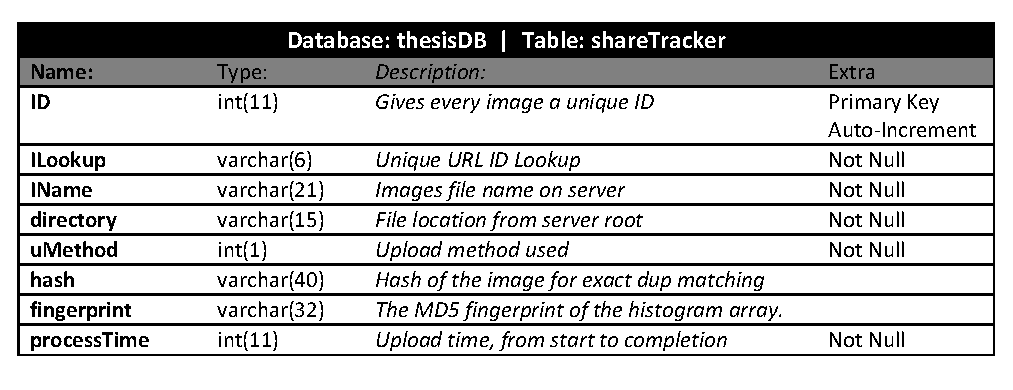
\includegraphics[width=6in]{schema}
\caption{Proposed schema for file uploads}
\label{fig:schema}
\end{figure}

In order to test the effectiveness of the research being discussed, a base case must be created against which to compare the results of running the algorithms. To create this data, the website performs one function before moving on to the duplicate reduction test. A separate directory was created on the server where every single image submission will be placed regardless of whether it is duplicate or not. This will mimic the upload process of a non-duplicate reducing image sharing website. Each entry into this folder will be placed in the database exactly the same as the duplicate reduced entries are, but will contain no image identification information. This first process is referenced henceforth as a traditional upload method. This upload method is unknown to the user as it will not return a URL allowing access to the image at a later time. During this process, each file is assigned a new, unique name to prevent collisions upon upload. A SQL {\tt "INSERT"} will then be run on the database for the image and will record the file's location on the server, the file name, the fact it was uploaded using the traditional method, the unique URL to access it from (which is not given to the user), and an {\tt ID} for each insert into the database. After the completion of the process an {\tt "UPDATE"} will be run on the database entry created by the {\tt "INSERT"} above. The time taken to complete the task will then be included in that entry and can be used to analyze the efficiency of both systems upon the completion of the tests outlined in section \ref{ch:reseval}.

After the initial upload completes, a second script is called. The second script has been designed to operate in two steps. This function performs mostly the same tasks as the traditional upload, but checks the image being uploaded for duplicates and handles each case appropriately. First, the image will be matched in the most basic form by hashing the image file using an MD5 file hashing function, after which the resulting hash will be compared to all images in the database using the following SQL Statement: {\tt "SELECT * FROM `share\_tracker' WHERE `uMethod' = `1' AND `hash' = `fileHash'"}. If this statement returns any results relating to a matching hash on a duplicate reduced uploaded image, it has found an exact matching image. 

In the event where a match is not found, the script will continue to the second stage of duplicate finding function. This function will operate in several different stages. The first stage toward finding an approximate image match is creating a fingerprint of the image file. In order to do this, the script will create a GD image object by using the PHP GD Image Library that was configured on the server in Section \ref{sec:serverconfig}. After the object is created, the GD Library has built in functions that allow iteration through every pixel in the image and view each pixel's red, green, blue value, or RGB value. These values will then be used to return a fingerprint in the form of an MD5 hash of the color frequency of the image. This color frequency is also known as a color profile. The next step to identifying a duplicate image would be to query the database for any images that have a perfectly matching color profile. This profile will be the same for an image no matter the variation as long as the image resolution, color and contrast are left unmodified. At this point, if there is no matching color profile, it can be said that there is most likely not a matching image on the server and
the function will return no matches found.

If the color profile does in fact match that of one or more images on the server, the script will then make a $16\times16$ pixel full color copy of the image being uploaded in addition to $16\times16$ copies of each of the images with a matching color profile. This process will also utilize functions provided by the GD Library that will allow pixel by pixel comparison of each image. When re-sizing an image, a number of techniques can be used when changing the total number of pixels. One popular method of re-sizing an image is called interpolation. With this process, when reducing the number of pixels, the algorithm will select one pixel and any immediate neighbors to it, at most there will be four. The algorithm will take the values of all five pixels and average them together eliminating the need for the neighbors as the original now represents the values of all five. This process is continued pixel by pixel until the image has reached its desired smaller dimension \cite{Acharya:2007}. This fact will allow the comparison of both images even if they were different dimensions, as the resulting $16\times16$ files will have similar averages after re-sizing if they are in fact a match. Because of a possibility of slight variations in color, this function will not look for exact match, but will allow a set amount of deviation between two thumbnails. To compare the pixels of both images, the RGB values of the corresponding pixels on each image will be analyzed. First, the red value of a pixel will be subtracted from the red value of the corresponding pixel's red value in the other thumbnail. The absolute value of the difference will be recorded. The same process will be completed for the green and blue values of that pixel. Once the difference from that pixel is calculated, the same comparison will be performed on each of the remaining pixels. In order to allow for very slight variations in color with each pixel, the resulting total calculated deviation will be divided by the number of pixels to `normalize' the result. After that calculation is complete, if the final deviation is less than or equal to the limit set by the website administrator, the function will return that a matching image was found.

If after all of the above processes are completed and no duplicate image is located on the server, the image upload will be accepted by the function and stored on the server's disk. At this time a SQL {\tt "INSERT"} will then be run on the database for the image and will record the file's long term location on the server, the file name, the fact that it was uploaded using the duplicate-reduced method, the unique URL to access it from, the image's MD5 hashed histogram that is described below, the thumbnail created for histogram comparison, and an {\tt ID} for each insert into the database. After the completion of the process an {\tt "UPDATE"} will be run on the database entry created by the {\tt "INSERT"} above. A view of the functioning duplicate-reduced upload process can be seen in figure \ref{success_nodupfound} when no duplicate image is located.

\begin{figure}[htbp]
\centering
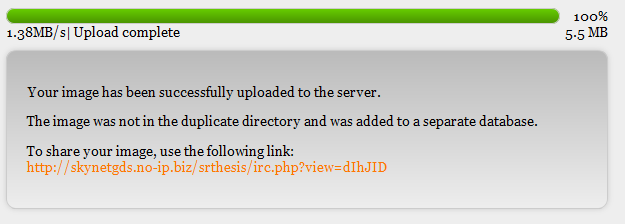
\includegraphics[width=5.5in]{success_nodupfound}
\caption{Successful image upload response when no duplicate is located.}
\label{success_nodupfound}
\end{figure}

If the image is determined to be a match after the completion of the full image hash function or the completion of the color profile and $16\times16$ pixel by pixel comparison, the submitted image is assumed to be a duplicate and a prompt will be displayed to the user showing the image they provided and the possible match that already exists. If the image is verified a match, the user will be given a unique link to the image that is already on the server, and the image being uploaded will be discarded as a duplicate. At this time the system will run an {\tt "INSERT"} on the database linking the new identifier to the image already on the server, and it will be added to the database. If the user decides the image is not a duplicate, the system will run an {\tt "INSERT"} statement and it will be added to the database. Following the completion of this process an {\tt "UPDATE"} will be run on the last {\tt "INSERT"} and the time taken to complete the task will be included in that entry. A view of the functioning duplicate-reduced upload process can be seen in figure \ref{success_dupfound} when a duplicate image is located.

\begin{figure}[htbp]
\centering
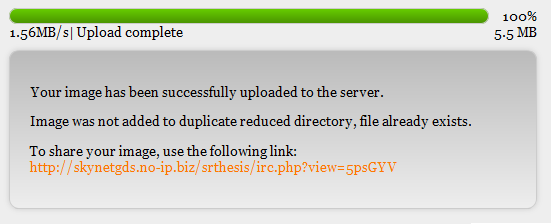
\includegraphics[width=5.5in]{success_dupfound}
\caption{Successful image upload response when a duplicate is located.}
\label{success_dupfound}
\end{figure}

In the case of requiring duplicate files, where the user decides to upload the image regardless of uniqueness, the script will be able to differentiate between the two images with the unique image ID that is generated at the time of insertion into the database. The closest matching occurrence of an image on the server compared to a new upload will be used in the prompt and displayed to the user. This will prevent frustration with multiple prompts every time more than one duplicate is found. This technique will also allow multiple links that point to the same image while leaving the user unaware of the system operating in the background to provide a consistent experience. An outline of this full process can be seen in figure \ref{method-fig1}.

\begin{figure}[htbp]
\centering
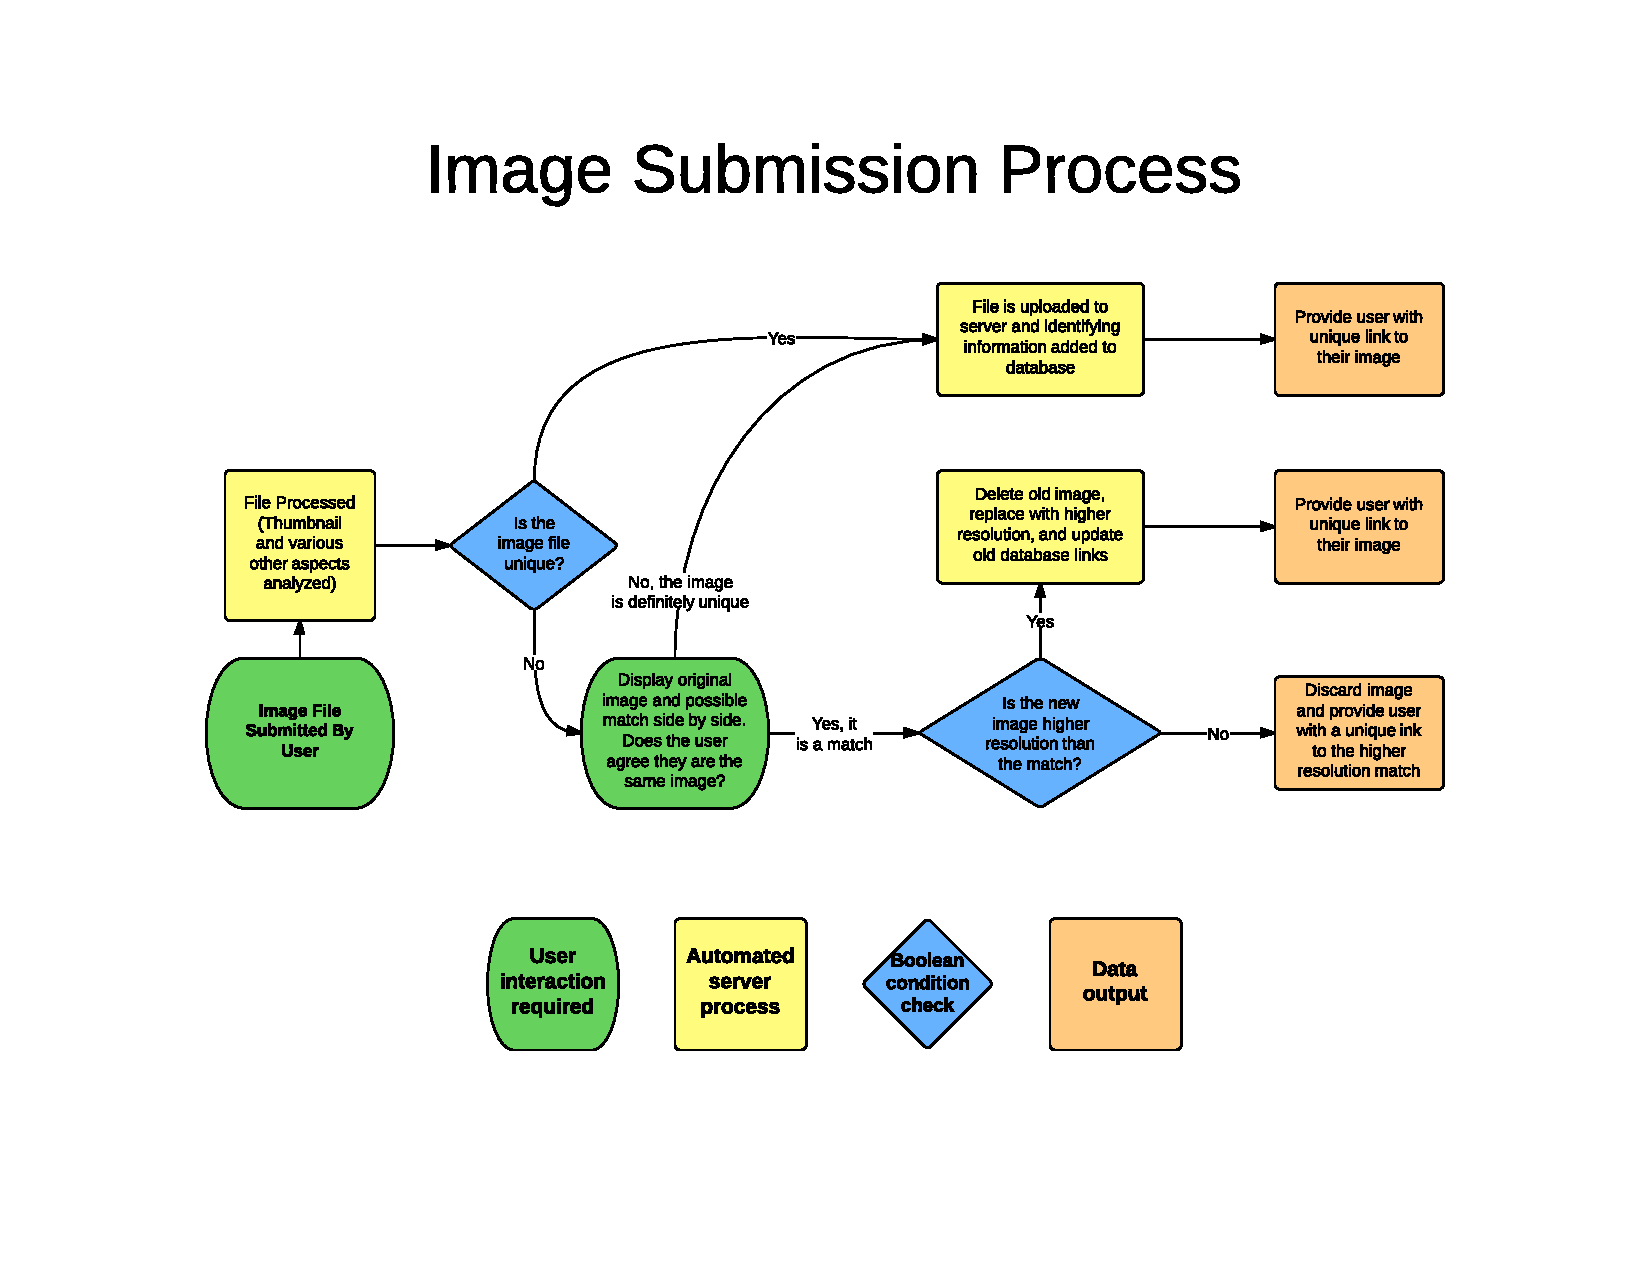
\includegraphics[trim={3cm 3.5cm 2cm 4.2cm},clip, width=6in]{upproc}
\caption{Streamlined upload process}
\label{method-fig1}
\end{figure}

When a user accesses the file from the provided link, the system will run a query that looks up the image identifier provided in the URL. If it matches an image on the server, the image location will be used to provide the image to the user for viewing. The user never notices a difference, but on the server side we have ensured file redundancy has been eliminated and possibly improved user experience by providing the user with higher quality content than what they were expecting. If the requested image is not found, a 404 ``Image cannot be found.'' error will be displayed to let the user know something went wrong.

\section{Color Profile and Histogram Comparison} \label{sec:histogram}
As mentioned in Section \ref{sec:websitedesign}, an image is composed of RGB values associated with every pixel in an image. In order to use these values in an effective manner, a thumbprint of the color profile had to be created. This color profile is represented as a histogram and allows the visualization of each color's frequency. This section will break down the process of comparing histograms and their accompanying data and explain the reasoning behind the comparison method chosen for this research.

As mentioned before, each pixel in an image is composed of an RGB value that allows the storage of the correct mixture of each color in that pixel. This value is separated into three separate ranges of 0-255 values where the higher the number the brighter the color. As seen in Figure \ref{historep}, a histogram has been generated using a popular photo editor by the name of Paint.NET. On the right hand side the four different overlaid histograms can be seen. The `x'-axis represents the relative number of occurrences of each 0-255 value while the `y'-axis represents the values themselves. The red layer indicates the frequency of each red value, the lowest of the 0-255 values being at the bottom of the image, and the highest at the top. The green and blue indicate the same for their respective colors. Also, note that blacks, whites, and grays can be represented by the RGB values. For example $255,255,255$ represents a solid white pixel while $000,000,000$ represents a pure black pixel, thus these colors do not require their own array.

\begin{figure}[htbp]
\centering
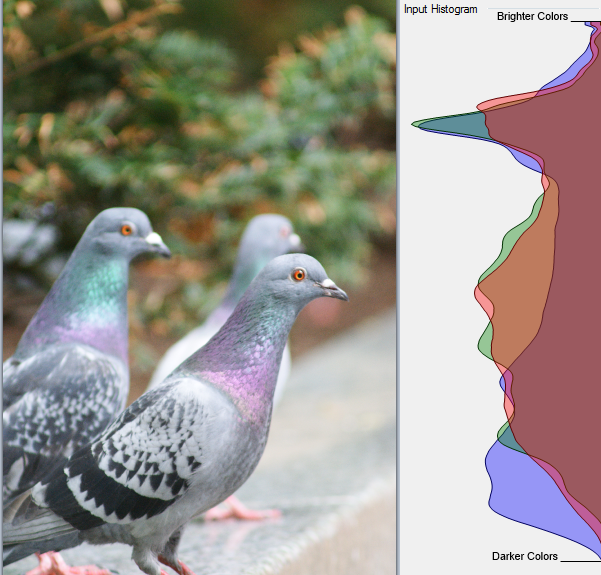
\includegraphics[width=4in]{historep}
\caption{Visual representation of an image's histogram}
\label{historep}
\end{figure}

This collection of values that make up the histogram is where the comparison process begins. For any comparison of data to occur, each pixel's RGB values must be recorded into three arrays of size 256. The index of the red, green, and blue arrays will correlate to the 256 possible colors within the respective color. As a color is encountered, a counter in the code will increment the value by one at that array index. This will allow the tracking of the frequency of each of the RGB values. It does not matter what pixel these are related to as the overall number and frequency of each color is the only concern.

At this point, every RGB value in the image should be stored within the color's respective array. This is the array of values that can be graphed using a histogram, and the visual of the color profile can be printed out for visual inspection. Since we will be using a function to process the values, the actual generation of said histogram would be unnecessary. These values can be handled and compared in a few ways, but the best method for the purpose of this research much be chosen. This array could be processed using the PHP {\tt serialize()} function and stored in the database for later examination. By doing this, each of the arrays would require separate serialization, and all three would require their own columns. With this method, the array could be pulled from the database and run through the {\tt deserialize()} function to return the array to its original state. This would be beneficial for applications that would require the comparison of each individual array index to another array. Due to the large amount of processing time required to iterate over multiple arrays of size 256, this is not optimal. In addition to this, we are not concerned with calculating the difference in color profiles, but are only concerned with an exact match. The use of exact-only matching is valuable with this research topic. If two images with different color profiles are being compared, it will be assumed that they are unique. An identical color profile could potentially signify a duplicate image as explained below.

The color profile requirement better lends itself to a different method of histogram value comparison. Due to the fact that we need to find only exact matches and that the system accounts for a possible false positive, hashing the three arrays will suffice. For this process, the three arrays will be concatenated in the order {\tt Red.Green.Blue}. This will generate one array with 1020 indexes representing the total relative count of each individual RGB color value. This value will then be taken and processed with the PHP $md5()$ function which will return a 40 character alphanumeric string representing the array. When an uploads fingerprint is created, the database will be searched for an exact match hash. If a matching hash is found, it is known that a photo with the same color profile is already on the server. In the event of a hash collision where two different histograms have the same resulting hash, the script will be performing a pixel by pixel comparison anyway and will be able to decide that the images are not unique, so this is not of concern.

Due to the fact that the only images of concern are exact color profile matches, it is not required to store the values of the color profile in a recoverable format. This leads away from storing either a plain text array of values in a database, or storing a serialized version of the array in the database. Because of this, it is acceptable for a 40 character alphanumeric hash to be stored in the database and directly compared to the hash of a newly submitted image in order to detect a possible duplicate image.

\section{Threats to Validity}  \label{sec:threats}
With any area of research comes inherent shortcomings no matter the care taken to eliminate free variables. By creating a locally hosted server and excluding any extraneous scripts from the website, these variables were controlled to the greatest extent possible. Due to the nature of a publicly hosted web server, there is always a chance of malicious attack which could skew the results one way or another. As discussed in Chapter \ref{ch:reseval}, four sets of experiments were performed. One test was performed offline using only a standard test image library with a very specific image alteration to each image. This environment gives the best possible chance of gathering unbiased results. The second test performed utilized the same image library, but was run over an internet connection instead of a LAN connection. This allowed for performance testing over a connection of fluctuating load and speed. An identical set of two experiments were tested using a set of 10 photographs taken around the Allegheny College campus during the winter months. This gives a collection of unique images, some of which would inherently have similar color profiles due to the reduced color intensity of the winter months.

Finally, the last variable that was not able to be determined was a possibility of image corruption. Due to the nature of images, it is possible that minor file corruption can occur on physical media. Since this is nothing more than the loss or incorrect representation of data, an image will still process using this system, but may yield incorrect results. In addition, if corruption occurs on a very small number of pixels, it is possible that the image will visually look identical to the original but still differ enough that it will be seen as an original image instead of a duplicate. This corruption can happen due to a momentarily lost connection, a web browser mishandling an HTTP request, or a server side fault. There are currently numerous open bugs in both the PHP language and the Apache server applications, none of which were researched to ensure the proper function of scripts. It was assumed that a functioning script returning expected results during trial runs is a fully operational script when running final tests and analyzing the results. % Discussion of how the topic was implemented

%ch:implem
%
% $Id: ch04_implementation.tex
%
%   *******************************************************************
%   * SEE THE MAIN FILE "AllegThesis.tex" FOR MORE INFORMATION.       *
%   *******************************************************************
%
\chapter{Results and Evaluation}\label{ch:reseval}
Another possible chapter title: Experimental Results
 % Chapter discussing the results and evaluations; inc threat to validity

%ch:conclusion
%
% $Id: conclusion.tex
%
%   *******************************************************************
%   * SEE THE MAIN FILE "AllegThesis.tex" FOR MORE INFORMATION.       *
%   *******************************************************************
%

\chapter{Discussion and Future Work}\label{ch:conclusion}

\section{Conclusion}
As discussed several times previously in this paper, image sharing websites can be extremely costly to operate as the service gains popularity and the number of images uploaded increases. The overall goal of any business owner is to cut costs and increase profits, and this is no different with owners of the image sharing websites in question. Through the use of various technologies including file expiration times, upload size restrictions, and subscription services the costs of running this type of service can be offset. Despite best efforts to reduce costs, further improvements could be implemented including the usage of this system. Although the method researched was unable to completely eliminate the duplicate data being uploaded to a server, it was able to eliminate 80-90\% of duplicates with a minimal number of false positives. As a worst case scenario, even removing a handful of duplicates from servers will leave business owners in a better position than not implementing the system at all. All of this was able to be accomplished with little to no additional effort on the users part, and a minimum additional wait time that was not observed to be more than two seconds in the worst scenario.

\section{Future Work}
In order to further develop a more versatile and accurate system, many improvements can be made. First and foremost, this research is limited strictly to JPEG images due to several code restrictions listed. Several image duplication detection algorithms exist that were discussed in the related works section. These can be used in place of the PHP GD library code based off of the system by CatPa \cite{catpa:gdcode}. In addition, the GD library does allow for additional file types, though the code will need optimized to maintain reasonable performance.

In addition to adding support for multiple file types, further research and optimization can be performed to increase the detection accuracy of the system developed. When analyzing photographs, the system performed as well as, or better than expected. This system performed exceptionally poorly with computer generated graphics, particularly patterns with a significant amount of detail. This could be accomplished using other detection techniques, altering this system's settings, or even furthering the detection process by adding a more thorough duplicate searching algorithm. Also, due to the fact that this research targeted only a finite set of image variations and manipulations, there is a need to test the systems accuracy on a wider variety of possible manipulations. This will not only give a better understanding of the overall performance, but it may open additional areas of improvement.

Finally, as discussed in Section \ref{sec:threats}, the sets of test images used in the experimentation and evaluation of this research were not complete enough to guarantee the findings would hold true in real world scenarios. These tests could include larger varieties of images or increased quantities, and would preferably cover a broader spectrum of possibilities allowing for better data to be collected. In addition, throughout the duration of this research, I was unable to locate a combination of files that would result in an MD5 hash collision that could cause false results to be returned. After generating and hashing nearly 300,000 images, each returned a unique file hash. Hash collisions are a known problem, though this scenario was unable to be tested after attempting to intentionally cause this sort of an unlikely event.

In conclusion, as with any type of research, the completion of a project does not signify the end of research on a particular topic, it only opens additional paths for further improvement. In the case of this research, versatility, performance, variance of image manipulations, handling of special situations, and further testing to give a better representation of real world performance are all areas that could benefit from further research. % Conclusion/future work

%   ********************************************************************
%   * IF YOU HAVE ANY APPENDICES (FOR INSTANCE, CODE, DATA, GRAPHS,    *
%   * OR ANYTHING ELSE THAT DOESN'T "FIT" AS REGULAR CHAPTER CONTENT), *
%   * INCLUDE THE FOLLOWING LINE, WHICH INSTRUCTS LATEX TO CHANGE FROM *
%   * NUMBERED "CHAPTER" HEADINGS TO LETTERED "APPENDIX" HEADINGS.     *
%   *                                                                  *
%   * APPENDICES HAVE THE SAME FORMATTING COMMANDS AS CHAPTERS (E.G.,  *
%   * "\chapter{...}", "\section{...}", ETC.)                          *
%   ********************************************************************

\appendix

%
% $Id: appa--code
%
%   *******************************************************************
%   * SEE THE MAIN FILE "AllegThesis.tex" FOR MORE INFORMATION.       *
%   *******************************************************************

\chapter{Duplicate Image Detection Code}\label{appa:didcode}
This appendix contains code relating directly to the uploading and duplicate image detection process. More precisely, the code relating to the exact image matching function is contained within Section \ref{appa:exact} while code relating to the more in-depth approximate duplicate image detection process is in Section \ref{appa:approx}.

\section{Upload Procedures}\label{appa:upload}
\lstinputlisting{Code/upload.php}

\section{Exact Duplicate Detection Code}\label{appa:exact}
\lstinputlisting{Code/dupFindSimple.php}

\section{Approximate Duplicate Detection Code}\label{appa:approx}
\lstinputlisting{Code/dupFindComplex.php}
\lstinputlisting{Code/phpDupeImage.php}

\chapter{Website Framework Code}\label{appb:wejbcode}
The code contained within this appendix describes only the research oriented
pages and supporting files that were 

%   *******************************************************************
%   * SEE THE MAIN FILE "AllegThesis.tex" FOR THE "\lstset" COMMAND   *
%   * THAT DEFINES HOW PROGRAM LISTINGS WILL LOOK.                    *
%   *******************************************************************

%\lstinputlisting{Code/SampleProg.java}

\chapter{Website Framework Code}\label{appb:webcode}
All program code should be fully commented. Authorship
of all parts of the code should be clearly specified. 

\chapter{Miscellaneous Code and Configurations}\label{appc:misccode}
  % Appendices to be included here

%   ********************************************************************
%   * THE FINAL COMMANDS DEAL WITH BIBLIOGRAPHY/REFERENCES. IF THERE   *
%   * ARE ANY ITEMS IN YOUR BIBTEX FILE THAT YOU DID NOT REFERENCE IN  *
%   * YOUR PAPER, BUT THAT YOU WISH TO INCLUDE IN THE BIBLIOGRAPHY,    *
%   * YOU MAY SPECIFY "\nocite" COMMANDS TO FORCE THEM TO BE INCLUDED. *
%   *                                                                  *
%   * THE COMMAND "\nocite{*}" FORCES EVERY ITEM IN YOUR BIBTEX FILE.  *
%   ********************************************************************

%\nocite{ckm-acmap-99}   % EXAMPLES OF FORCING THINGS TO BE INCLUDED
%\nocite{Dierckx93}      %   "   "   "
%\nocite{obs-stcav-92}   %   "   "   "
%\nocite{bb4471}         %   "   "   "

\nocite{*} % OR DO THIS TO INCLUDE ALL BIBTEX REFERENCES IN THE BIBLIOGRAPHY

\bibliographystyle{plain}

%   ********************************************************************
%   * IF YOU HAVE YOUR BIBLIOGRAPHY IN A SEPARATE ".bib" FILE, HERE IS *
%   * WHERE YOU MUST SPECIFY IT. IN THIS EXAMPLE, THE BIBLIOGRAPHY     *
%   * ENTRIES ARE STORED IN A SUBDIRECTORY NAMED "Bibdir" IN A FILE    *
%   * NAMED "myBibtexDB.bib".                                          *
%   ********************************************************************

\begin{spacing}{1}
\bibliography{Bibdir/myBibtexDB}    % File type ".bib" is assumed
\end{spacing}

%   ********************************************************************
%   * THIS FEATURE HAS BEEN DISABLED:                                  *
%   ********************************************************************
% \include{colophon}

\typeout{THEPAGE \thepage}

\end{document}
